\subsubsection{Temperatur-Senosr} \label{temp-1}

Für das Projekt wurde zu Beginn ein Infrarot-Temperatursensor des Typs MLX90614 von der Firma Melexis-Microelectronic Integrated Systems verwendet. Der MLX90614 ist ein sensibler digitaler  16-Bit Sensor, dessen Genauigkeit bei +-0,5C liegt. Der Arbeitsbereich ist für Temperaturen des Sensors liegt zwischen -40C und +125C, und für die Kontaktlose Messung an Objekten, also der mögliche Temperatur Messbereich, zwischen -40C und +380C. Die Datenübertragung vom Sensor auf das Messboard erfolgt mittels eines I2C-Busses (siehe Abschnitt x.x zu I2C). Die Übertragungsrate wurde hierbei mit 100.000 kbit/s gewählt. Die Verwendung von I2C hat den Vorteil, dass auch andere digitale Sensoren ohne größeren zusätzlichen verkabelungs- Aufwand an den Bus angeschlossen werden können. In der Abbildung X ist der Anschluss des Sensor exemplarisch aufgezeigt.

\begin{figure}[H] \centering
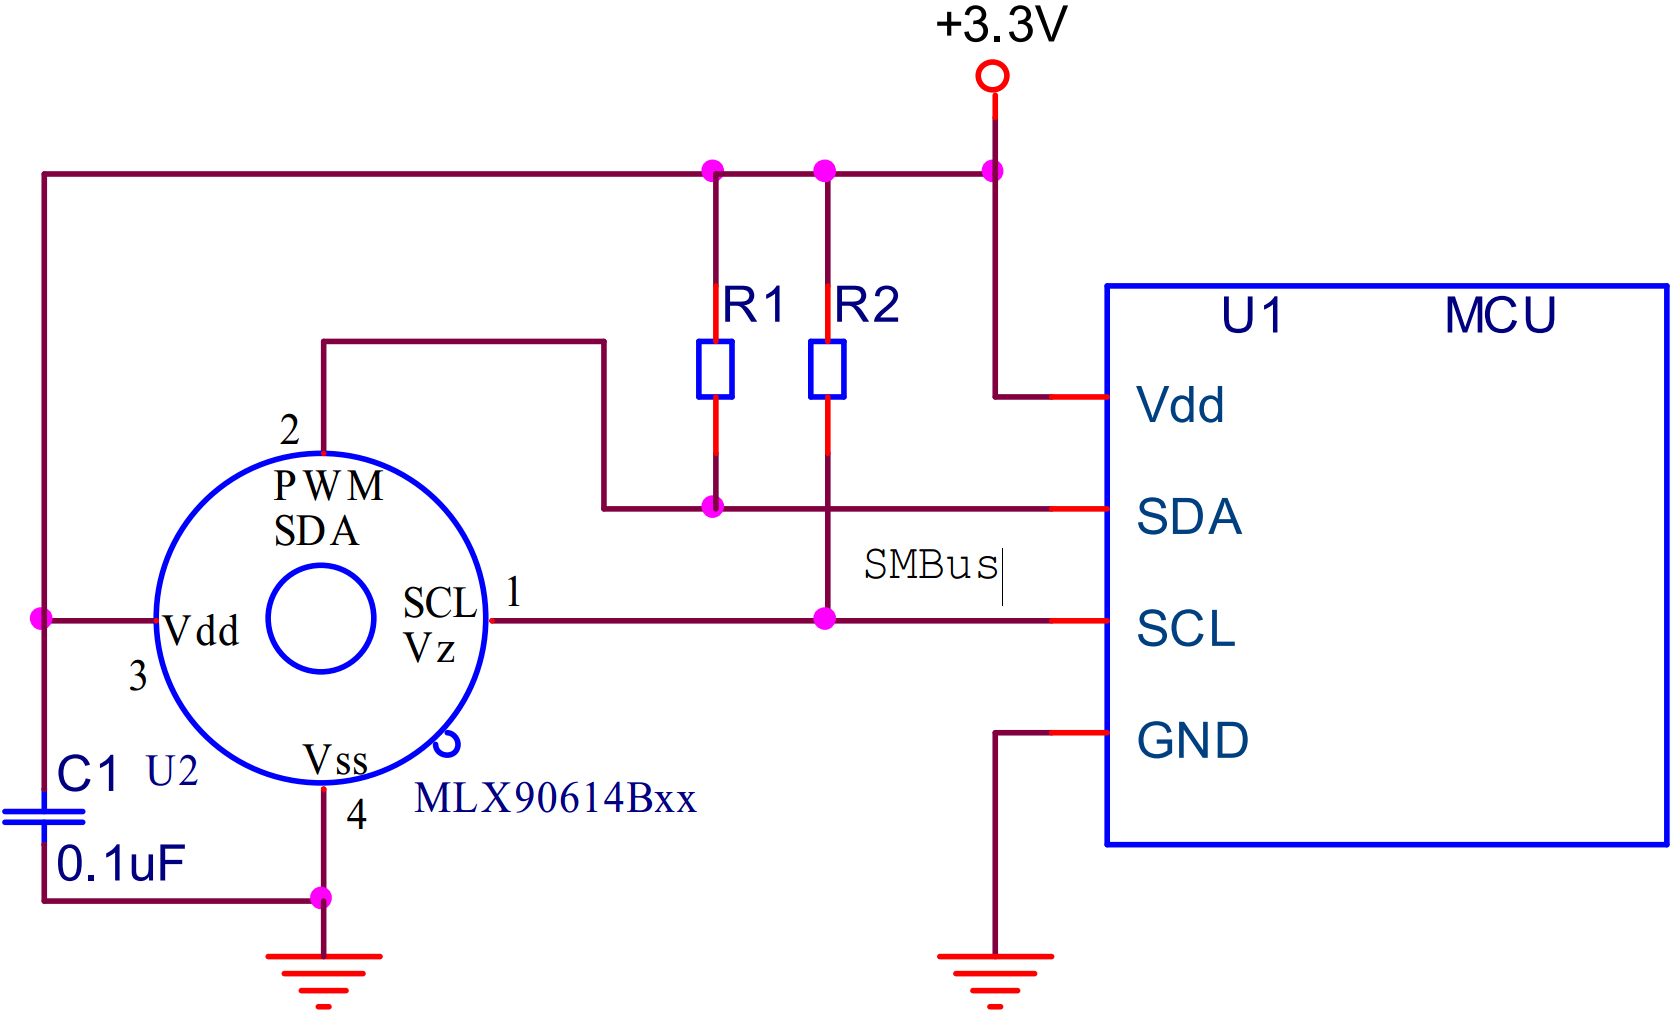
\includegraphics[width=\textwidth]{Images/Temp_Sensor.png} 
\vspace{-0.3cm} 
\caption{Abb.  Verbindung des Temperatursensors nach Datenblatt.}
\label{fig-elise} 
\end{figure}

Die Auswahl dieses Sensors beruhte maßgeblich auf dem Messprinzip der Infrarot Messung. Es ist zwar auch möglich Temperaturen mittels Sensoren zu messen, die auf Kontakt mit dem Messobjekt beruhen. Etwa durch ein Messprinzip, dass auf der Änderung des Wiederstandes des Messkörpers beruht. Das Problem dieser Sensortypen ist allerdings, dass Änderungen der Temperatur am Messobjekt ein gewisse Verzögerung der Messung hervorrufen, da der Sensor selbst erst einmal die geänderte Temperatur annehmen muss. Bei einer Messung mit Infrarot ist kein Kontakt mit dem Messobjekt nötig, und Änderungen der Temperatur werden sofort erkannt. Somit ermöglicht der MLX90614 mit seiner Infrarotmessung die Erkennung von kleineren und kurzfristigeren Temperaturschwankungen.

Der MLX90614 wurde durchgehend für das gesamte Projekt in allen Prototypen genutzt. Es sei an dieser Stelle allerdings erwähnt, dass im Projekt ausschließlich die Ausführung mit dem Plastikgehäuse verwendet wurde. Es wurde zwar auch eine Variante mit Metallgehäuse getestet, allerdings gab es dort Probleme, wenn dieser in direktem Kontakt mit der Haut war. Das Problem beruht auf der sehr starken Erhitzung des Gehäuses, das vermutlich durch einen Kurzschluss des Vdd-Pins mit dem Gehäuse(Masse-Pin) zustande kam. Eine zusätzliche Isolierung der Pins durch Schrumpfschläuche, sowie die Isolierung des Gehäuses von den Pins mittels Epoxidharzklebstoffs konnten hier keine Abhilfe schaffen. Das Problem tritt bei Sensoren mit Plastikgehäuse schlicht nicht auf, weswegen der in Abbildung y gezeigte Sensor bei allen Messungen und Prototypen zum Einsatz kam.

\begin{figure}[H] \centering
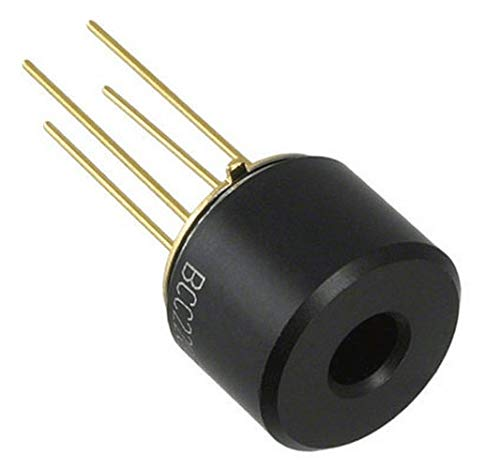
\includegraphics[width=\textwidth]{Images/Temp_Case.png} 
\vspace{-0.3cm} 
\caption{Abb. Temperatur-Sensor MLX90614 mit Plastikgehäuse}
\label{fig-elise} 
\end{figure}




